\section{Re-running the published configuration}
\label{sec:results}

\paragraph{The released script.}
We ran the released \texttt{EEGclassify.py} with the README command (seed 42) on our hardware
(Appendix~\ref{app:upstream}). It printed 9.69\%. This is the highest of its 313 evaluation-set
accuracies, reached in epoch 66; we checked that the printed value equals the maximum of the logged
curve. The last checkpoint scored 7.77\%, and evaluation accuracy after the 10-epoch warm-up averaged
7.40\% (SD 0.84). The published 13.88\% is 4.2 points above the best value this run reached.

\paragraph{Our re-implementation matches the released script.}
With the same configuration, the per-epoch training loss of our re-implementation differs from
that of the released script by at most 0.043 (mean 0.016) across three seeds, ending at 3.37--3.40 against
3.40, and the evaluation curves overlap (Appendix Figure~\ref{fig:upstream}). Under the published rule it scores 8.75\% $\pm$ 0.67 over three
seeds (8.33, 8.41, 9.53), against 9.69\% for the released script's single seed. Neither reaches
13.88\%. We do not know what accounts for the remaining difference; candidates include hardware,
seed, and software versions, and we could not test the authors' environment.

\paragraph{Three selection rules, real and permuted labels.}
Table~\ref{tab:repro} reads three rules from the same runs. Taking the best of 281 evaluations gives
8.75\% with real labels and 6.38\% with permuted training labels; the permuted value is 0.9 points
above the paper's own shuffled baseline (5.52\%), which used the same rule. Choosing the checkpoint on
held-out validation data instead gives 7.13\% and 5.02\%, and the last checkpoint 7.39\% and 4.80\%.
The max rule therefore adds 1.6 points to the real-label result and 1.4 to the permuted one; in both
cases the maximum sits above the average over all post-warm-up evaluations (7.01\% real, 5.02\%
permuted) by 1.75 and 1.35 points (Figure~\ref{fig:curves}). Real labels beat permuted labels by 2.1
to 2.6 points under every rule. The published margin is 8.4.

\begin{table}[t]
\centering
\small
\caption{\textbf{One configuration, three readings.} Accuracy (\%) on the released evaluation set
(1{,}249 trials) for the published configuration (500\,Hz, 100 epochs), mean $\pm$ SD over three
seeds, read from the same runs under three selection rules. Permuted: training labels shuffled,
evaluation labels intact. The 95\% CI for the no-EEG classifier is a run-clustered bootstrap.
Source: \texttt{results/summary.json}, generated by \texttt{scripts/generate\_tables.py}.}
\label{tab:repro}
\begin{tabular}{lccc}
\toprule
Selection rule & Real labels & Permuted training labels & Difference \\
\midrule
Max over checkpoints (published rule) & 8.75 $\pm$ 0.67 & 6.38 $\pm$ 0.30 & 2.38 \\
Validation-selected checkpoint & 7.13 $\pm$ 0.24 & 5.02 $\pm$ 0.76 & 2.11 \\
Last checkpoint & 7.39 $\pm$ 0.73 & 4.80 $\pm$ 0.70 & 2.59 \\
\midrule
Released script, seed 42, max over checkpoints & 9.69 & -- & -- \\
Released script, seed 42, last checkpoint & 7.77 & -- & -- \\
Published \citep[Table 3, S1]{zhang2024chisco} & 13.88 & 5.52 & 8.36 \\
\midrule
No EEG: label of previous training trial & \multicolumn{3}{l}{18.82 (95\% CI 16.49--21.57)} \\
No EEG: majority class & \multicolumn{3}{l}{4.72} \\
Uniform chance ($1/39$) & \multicolumn{3}{l}{2.56} \\
\bottomrule
\end{tabular}

\end{table}


\begin{figure}[t]
  \centering
  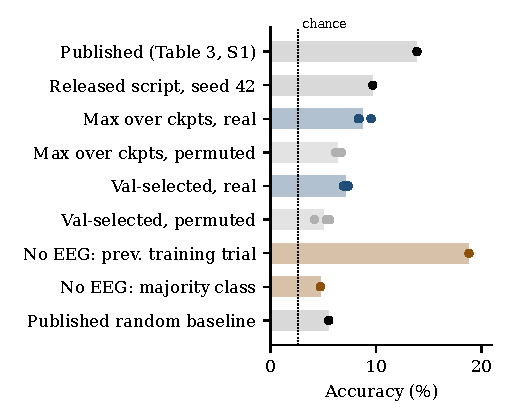
\includegraphics[width=0.49\linewidth]{figures/fig_main.pdf}\hfill
  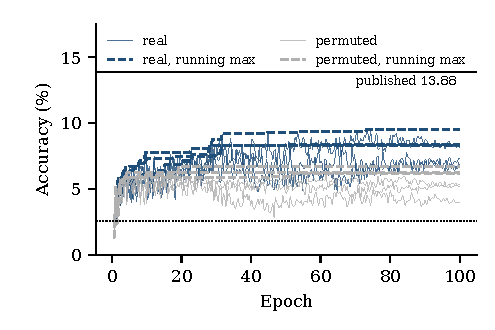
\includegraphics[width=0.49\linewidth]{figures/fig_curves.pdf}
  \caption{\textbf{Left:} accuracy on the released evaluation set. Bars are means, dots are seeds;
  ``Max over ckpts'' is the published selection rule, ``Val-selected'' the checkpoint with the best
  held-out validation accuracy; the brown bars use no EEG. \textbf{Right:} evaluation-set accuracy
  at each of the 281 evaluations of the published configuration (three seeds each), with running
  maxima (dashed); the published rule reports the end point of the dashed line.
  Source: \texttt{results/imagine\_full\_500hz\_interleaved\_*\_e100\_seed*.json}.}
  \label{fig:curves}
\end{figure}

\paragraph{Does the EEG model use the order structure?}
On the released split, the nearest earlier training trial shares the evaluation trial's category for
18.8\% of evaluation trials. At the validation-selected checkpoint, real-label models predict that
neighbour's category for 6.5--7.6\% of evaluation trials, 2.4--3.7 points more than their own class
frequencies would produce if predictions were independent of the neighbour (3.8--4.1\%).
Permuted-label models show no excess (4.1--4.6\% observed vs.\ 4.4--4.6\% expected). Real-label
accuracy is 11.8\% on trials whose neighbour shares the category and 6.0\% on the rest; for permuted
labels the corresponding values are 6.8\% and 4.6\%, so part of this gap reflects class frequency
rather than neighbour copying. The trials whose neighbour differs are not leak-free either:
predicting the most common training category of the trial's run scores 10.7\% on them without EEG.
On the released split, then, the real-label model's advantage over its null is at least partly
mediated by the recording-time structure that the no-EEG classifiers exploit. Whether any advantage
remains without that structure is the question of the next section.

\section{Changing the split}
\label{sec:splits}

We trained the same model under four splits, each with real and permuted training labels
(Table~\ref{tab:splits}, Figure~\ref{fig:splits}; 250\,Hz, 30 epochs, three seeds, three folds per
seed for grouped splits).

\paragraph{The real-vs-permuted margin shrinks as neighbours are removed.}
With the validation-selected checkpoint, real labels beat permuted labels by 2.11 points on the
released split and 1.01 on a random-trial split, both of which leave nearly every evaluation trial
with training neighbours from its own run (the position-only classifier scores 18.82\% and 18.25\% on
them). Holding out whole runs removes those neighbours: accuracy falls to 4.37\% for real labels and
3.73\% for permuted labels, a difference of 0.64 points. Paired by seed and fold, real labels are
ahead in 7 of 9 comparisons, with differences from $-2.42$ to $+2.71$ points; the mean difference is
about the size of the seed-to-seed standard deviation (0.49 real, 0.60 permuted). With three seeds
and three folds we cannot distinguish a residual signal of this size from none. Holding out a whole
recording day gives 2.55\% and 2.75\%, both at uniform chance; because the category mix differs
between days (Appendix~\ref{app:data}), we do not interpret this split further.

\paragraph{The published rule produces above-chance numbers without information.}
Under session holdout, where the validation-selected checkpoint is at chance for both conditions,
taking the best evaluation-set accuracy over training reports 5.66\% for real labels and 5.26\% for
permuted labels, more than double uniform chance. Under run holdout the same rule reports 6.27\% and
5.37\%. A best-of-many-evaluations number on the evaluation set is therefore not a reliable
indicator of decoding, even when the split itself is sound.

\begin{table}[t]
\centering
\small
\caption{\textbf{Split comparison} (accuracy, \%; 250\,Hz, 30 epochs). EEG columns: mean $\pm$ SD
over three seeds; for run and session holdout each seed's value is the mean over three held-out
folds. No-EEG columns are computed on exactly the same evaluation folds. Source:
\texttt{results/summary.json}.}
\label{tab:splits}
\setlength{\tabcolsep}{4pt}
\begin{tabular}{lccccc}
\toprule
 & \multicolumn{3}{c}{EEG model} & \multicolumn{2}{c}{No EEG} \\
\cmidrule(lr){2-4}\cmidrule(lr){5-6}
Split & Real & Permuted & Difference & Prev.\ trial & Majority \\
\midrule
\multicolumn{6}{l}{\emph{Validation-selected checkpoint}} \\
Interleaved (released) & 7.58 $\pm$ 1.04 & 5.47 $\pm$ 0.48 & 2.11 & 18.82 & 4.72 \\
Random trial & 5.79 $\pm$ 1.24 & 4.78 $\pm$ 0.53 & 1.01 & 18.25 & 4.70 \\
Run holdout & 4.37 $\pm$ 0.49 & 3.73 $\pm$ 0.60 & 0.64 & 4.02 & 3.36 \\
Session holdout & 2.55 $\pm$ 0.13 & 2.75 $\pm$ 0.43 & $-$0.20 & 3.28 & 2.58 \\
\multicolumn{6}{l}{\emph{Max over checkpoints (published rule)}} \\
Interleaved (released) & 8.17 $\pm$ 0.24 & 6.06 $\pm$ 0.18 & 2.11 &  &  \\
Random trial & 6.99 $\pm$ 0.88 & 5.20 $\pm$ 0.37 & 1.79 &  &  \\
Run holdout & 6.27 $\pm$ 0.08 & 5.37 $\pm$ 0.76 & 0.90 &  &  \\
Session holdout & 5.66 $\pm$ 1.22 & 5.26 $\pm$ 0.54 & 0.40 &  &  \\
\bottomrule
\end{tabular}

\end{table}

\begin{figure}[t]
  \centering
  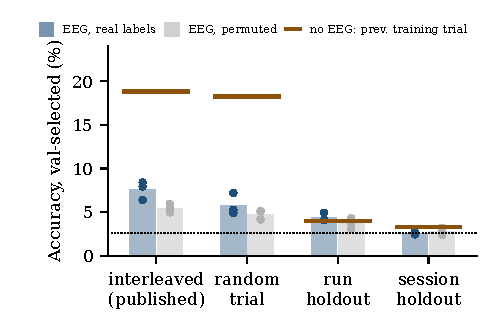
\includegraphics[width=0.62\linewidth]{figures/fig_splits.pdf}
  \caption{\textbf{Holding out whole runs.} Validation-selected accuracy by split for real (blue)
  and permuted (grey) training labels; dots are seeds. Brown lines: the position-only classifier on
  the same evaluation folds. Dotted line: uniform chance (2.56\%).}
  \label{fig:splits}
\end{figure}

\paragraph{Reading-task positive control.}
To see how much this pipeline can detect once recording-time cues are removed, we trained the same
model on the reading epochs of the same trials (Table~\ref{tab:read}). Reading is a visual task, and
we expected it to be at least as decodable as imagination. On the released split, reading scores
6.99\%, slightly below imagined speech (7.58\%). Under run holdout it scores 4.85\% against 3.75\% for
permuted labels, a difference of 1.10 points; real labels are ahead in 7 of 9 seed-fold pairs
(range $-0.46$ to $+4.34$), and most of the difference comes from one of the three held-out folds.
The pipeline therefore has limited sensitivity to category information when the order structure is
removed, for reading as well as for imagination. The small run-holdout margin for imagined speech
should be read with that in mind: it is weak evidence in either direction, not evidence of absence.

\begin{table}[t]
\centering
\small
\caption{\textbf{Reading-task control} (validation-selected accuracy, \%; 250\,Hz, 30 epochs; 6{,}387
reading epochs of 5\,s). The last column repeats the imagined-speech difference from
Table~\ref{tab:splits} for comparison. The permuted-label reading model was run only for run
holdout.}
\label{tab:read}
\begin{tabular}{lcccc}
\toprule
Task, split & Real & Permuted & Difference & Imagined: difference \\
\midrule
Reading, interleaved (released) & 6.99 $\pm$ 0.53 & not run & -- & 2.11 \\
Reading, run holdout & 4.85 $\pm$ 0.40 & 3.75 $\pm$ 0.54 & 1.10 & 0.64 \\
\bottomrule
\end{tabular}

\end{table}
